
%% bare_conf.tex
%% V1.4b
%% 2015/08/26
%% by Michael Shell
%% See:
%% http://www.michaelshell.org/
%% for current contact information.
%%
%% This is a skeleton file demonstrating the use of IEEEtran.cls
%% (requires IEEEtran.cls version 1.8b or later) with an IEEE
%% conference paper.
%%
%% Support sites:
%% http://www.michaelshell.org/tex/ieeetran/
%% http://www.ctan.org/pkg/ieeetran
%% and
%% http://www.ieee.org/

%%*************************************************************************
%% Legal Notice:
%% This code is offered as-is without any warranty either expressed or
%% implied; without even the implied warranty of MERCHANTABILITY or
%% FITNESS FOR A PARTICULAR PURPOSE! 
%% User assumes all risk.
%% In no event shall the IEEE or any contributor to this code be liable for
%% any damages or losses, including, but not limited to, incidental,
%% consequential, or any other damages, resulting from the use or misuse
%% of any information contained here.
%%
%% All comments are the opinions of their respective authors and are not
%% necessarily endorsed by the IEEE.
%%
%% This work is distributed under the LaTeX Project Public License (LPPL)
%% ( http://www.latex-project.org/ ) version 1.3, and may be freely used,
%% distributed and modified. A copy of the LPPL, version 1.3, is included
%% in the base LaTeX documentation of all distributions of LaTeX released
%% 2003/12/01 or later.
%% Retain all contribution notices and credits.
%% ** Modified files should be clearly indicated as such, including  **
%% ** renaming them and changing author support contact information. **
%%*************************************************************************


% *** Authors should verify (and, if needed, correct) their LaTeX system  ***
% *** with the testflow diagnostic prior to trusting their LaTeX platform ***
% *** with production work. The IEEE's font choices and paper sizes can   ***
% *** trigger bugs that do not appear when using other class files.       ***                          ***
% The testflow support page is at:
% http://www.michaelshell.org/tex/testflow/



\documentclass[conference]{IEEEtran}\linespread{0.9} 
\usepackage{graphicx}
\usepackage{tabularx}
\usepackage{algorithm}
\usepackage{algpseudocode}
\usepackage{fancyhdr}
% Some Computer Society conferences also require the compsoc mode option,
% but others use the standard conference format.
%
% If IEEEtran.cls has not been installed into the LaTeX system files,
% manually specify the path to it like:
% \documentclass[conference]{../sty/IEEEtran}

\thispagestyle{plain}
\pagestyle{fancy}

\fancyhf{}
\fancyfoot[C]{\fontsize{11}{0}\selectfont 2017 Seventh International Symposium on Embedded Computing and System Design (ISED)}
\renewcommand{\footrulewidth}{0pt}

\usepackage{eso-pic}
\usepackage{xcolor}


% Some very useful LaTeX packages include:
% (uncomment the ones you want to load)


% *** MISC UTILITY PACKAGES ***
%
%\usepackage{ifpdf}
% Heiko Oberdiek's ifpdf.sty is very useful if you need conditional
% compilation based on whether the output is pdf or dvi.
% usage:
% \ifpdf
%   % pdf code
% \else
%   % dvi code
% \fi
% The latest version of ifpdf.sty can be obtained from:
% http://www.ctan.org/pkg/ifpdf
% Also, note that IEEEtran.cls V1.7 and later provides a builtin
% \ifCLASSINFOpdf conditional that works the same way.
% When switching from latex to pdflatex and vice-versa, the compiler may
% have to be run twice to clear warning/error messages.






% *** CITATION PACKAGES ***
%
%\usepackage{cite}
% cite.sty was written by Donald Arseneau
% V1.6 and later of IEEEtran pre-defines the format of the cite.sty package
% \cite{} output to follow that of the IEEE. Loading the cite package will
% result in citation numbers being automatically sorted and properly
% "compressed/ranged". e.g., [1], [9], [2], [7], [5], [6] without using
% cite.sty will become [1], [2], [5]--[7], [9] using cite.sty. cite.sty's
% \cite will automatically add leading space, if needed. Use cite.sty's
% noadjust option (cite.sty V3.8 and later) if you want to turn this off
% such as if a citation ever needs to be enclosed in parenthesis.
% cite.sty is already installed on most LaTeX systems. Be sure and use
% version 5.0 (2009-03-20) and later if using hyperref.sty.
% The latest version can be obtained at:
% http://www.ctan.org/pkg/cite
% The documentation is contained in the cite.sty file itself.






% *** GRAPHICS RELATED PACKAGES ***
%
\ifCLASSINFOpdf
  % \usepackage[pdftex]{graphicx}
  % declare the path(s) where your graphic files are
  % \graphicspath{{../pdf/}{../jpeg/}}
  % and their extensions so you won't have to specify these with
  % every instance of \includegraphics
  % \DeclareGraphicsExtensions{.pdf,.jpeg,.png}
\else
  % or other class option (dvipsone, dvipdf, if not using dvips). graphicx
  % will default to the driver specified in the system graphics.cfg if no
  % driver is specified.
  % \usepackage[dvips]{graphicx}
  % declare the path(s) where your graphic files are
  % \graphicspath{{../eps/}}
  % and their extensions so you won't have to specify these with
  % every instance of \includegraphics
  % \DeclareGraphicsExtensions{.eps}
\fi
% graphicx was written by David Carlisle and Sebastian Rahtz. It is
% required if you want graphics, photos, etc. graphicx.sty is already
% installed on most LaTeX systems. The latest version and documentation
% can be obtained at: 
% http://www.ctan.org/pkg/graphicx
% Another good source of documentation is "Using Imported Graphics in
% LaTeX2e" by Keith Reckdahl which can be found at:
% http://www.ctan.org/pkg/epslatex
%
% latex, and pdflatex in dvi mode, support graphics in encapsulated
% postscript (.eps) format. pdflatex in pdf mode supports graphics
% in .pdf, .jpeg, .png and .mps (metapost) formats. Users should ensure
% that all non-photo figures use a vector format (.eps, .pdf, .mps) and
% not a bitmapped formats (.jpeg, .png). The IEEE frowns on bitmapped formats
% which can result in "jaggedy"/blurry rendering of lines and letters as
% well as large increases in file sizes.
%
% You can find documentation about the pdfTeX application at:
% http://www.tug.org/applications/pdftex





% *** MATH PACKAGES ***
%
%\usepackage{amsmath}
% A popular package from the American Mathematical Society that provides
% many useful and powerful commands for dealing with mathematics.
%
% Note that the amsmath package sets \interdisplaylinepenalty to 10000
% thus preventing page breaks from occurring within multiline equations. Use:
%\interdisplaylinepenalty=2500
% after loading amsmath to restore such page breaks as IEEEtran.cls normally
% does. amsmath.sty is already installed on most LaTeX systems. The latest
% version and documentation can be obtained at:
% http://www.ctan.org/pkg/amsmath





% *** SPECIALIZED LIST PACKAGES ***
%
%\usepackage{algorithmic}
% algorithmic.sty was written by Peter Williams and Rogerio Brito.
% This package provides an algorithmic environment fo describing algorithms.
% You can use the algorithmic environment in-text or within a figure
% environment to provide for a floating algorithm. Do NOT use the algorithm
% floating environment provided by algorithm.sty (by the same authors) or
% algorithm2e.sty (by Christophe Fiorio) as the IEEE does not use dedicated
% algorithm float types and packages that provide these will not provide
% correct IEEE style captions. The latest version and documentation of
% algorithmic.sty can be obtained at:
% http://www.ctan.org/pkg/algorithms
% Also of interest may be the (relatively newer and more customizable)
% algorithmicx.sty package by Szasz Janos:
% http://www.ctan.org/pkg/algorithmicx




% *** ALIGNMENT PACKAGES ***
%
%\usepackage{array}
% Frank Mittelbach's and David Carlisle's array.sty patches and improves
% the standard LaTeX2e array and tabular environments to provide better
% appearance and additional user controls. As the default LaTeX2e table
% generation code is lacking to the point of almost being broken with
% respect to the quality of the end results, all users are strongly
% advised to use an enhanced (at the very least that provided by array.sty)
% set of table tools. array.sty is already installed on most systems. The
% latest version and documentation can be obtained at:
% http://www.ctan.org/pkg/array


% IEEEtran contains the IEEEeqnarray family of commands that can be used to
% generate multiline equations as well as matrices, tables, etc., of high
% quality.




% *** SUBFIGURE PACKAGES ***
%\ifCLASSOPTIONcompsoc
%  \usepackage[caption=false,font=normalsize,labelfont=sf,textfont=sf]{subfig}
%\else
%  \usepackage[caption=false,font=footnotesize]{subfig}
%\fi
% subfig.sty, written by Steven Douglas Cochran, is the modern replacement
% for subfigure.sty, the latter of which is no longer maintained and is
% incompatible with some LaTeX packages including fixltx2e. However,
% subfig.sty requires and automatically loads Axel Sommerfeldt's caption.sty
% which will override IEEEtran.cls' handling of captions and this will result
% in non-IEEE style figure/table captions. To prevent this problem, be sure
% and invoke subfig.sty's "caption=false" package option (available since
% subfig.sty version 1.3, 2005/06/28) as this is will preserve IEEEtran.cls
% handling of captions.
% Note that the Computer Society format requires a larger sans serif font
% than the serif footnote size font used in traditional IEEE formatting
% and thus the need to invoke different subfig.sty package options depending
% on whether compsoc mode has been enabled.
%
% The latest version and documentation of subfig.sty can be obtained at:
% http://www.ctan.org/pkg/subfig




% *** FLOAT PACKAGES ***
%
%\usepackage{fixltx2e}
% fixltx2e, the successor to the earlier fix2col.sty, was written by
% Frank Mittelbach and David Carlisle. This package corrects a few problems
% in the LaTeX2e kernel, the most notable of which is that in current
% LaTeX2e releases, the ordering of single and double column floats is not
% guaranteed to be preserved. Thus, an unpatched LaTeX2e can allow a
% single column figure to be placed prior to an earlier double column
% figure.
% Be aware that LaTeX2e kernels dated 2015 and later have fixltx2e.sty's
% corrections already built into the system in which case a warning will
% be issued if an attempt is made to load fixltx2e.sty as it is no longer
% needed.
% The latest version and documentation can be found at:
% http://www.ctan.org/pkg/fixltx2e


%\usepackage{stfloats}
% stfloats.sty was written by Sigitas Tolusis. This package gives LaTeX2e
% the ability to do double column floats at the bottom of the page as well
% as the top. (e.g., "\begin{figure*}[!b]" is not normally possible in
% LaTeX2e). It also provides a command:
%\fnbelowfloat
% to enable the placement of footnotes below bottom floats (the standard
% LaTeX2e kernel puts them above bottom floats). This is an invasive package
% which rewrites many portions of the LaTeX2e float routines. It may not work
% with other packages that modify the LaTeX2e float routines. The latest
% version and documentation can be obtained at:
% http://www.ctan.org/pkg/stfloats
% Do not use the stfloats baselinefloat ability as the IEEE does not allow
% \baselineskip to stretch. Authors submitting work to the IEEE should note
% that the IEEE rarely uses double column equations and that authors should try
% to avoid such use. Do not be tempted to use the cuted.sty or midfloat.sty
% packages (also by Sigitas Tolusis) as the IEEE does not format its papers in
% such ways.
% Do not attempt to use stfloats with fixltx2e as they are incompatible.
% Instead, use Morten Hogholm'a dblfloatfix which combines the features
% of both fixltx2e and stfloats:
%
% \usepackage{dblfloatfix}
% The latest version can be found at:
% http://www.ctan.org/pkg/dblfloatfix




% *** PDF, URL AND HYPERLINK PACKAGES ***
%
%\usepackage{url}
% url.sty was written by Donald Arseneau. It provides better support for
% handling and breaking URLs. url.sty is already installed on most LaTeX
% systems. The latest version and documentation can be obtained at:
% http://www.ctan.org/pkg/url
% Basically, \url{my_url_here}.




% *** Do not adjust lengths that control margins, column widths, etc. ***
% *** Do not use packages that alter fonts (such as pslatex).         ***
% There should be no need to do such things with IEEEtran.cls V1.6 and later.
% (Unless specifically asked to do so by the journal or conference you plan
% to submit to, of course. )


% correct bad hyphenation here
\hyphenation{op-tical net-works semi-conduc-tor}


\IEEEoverridecommandlockouts
\IEEEpubid{\makebox[\columnwidth]{978-1-5386-3032-7/17/\$31.00~\copyright~2017 IEEE \hfill} 
\hspace{\columnsep}
\makebox[\columnwidth]{ }}

\begin{document}
%\AddToShipoutPictureBG*{%
%  \AtPageLowerLeft{%
%    \setlength\unitlength{1in}%
%    \hspace*{\dimexpr0.5\paperwidth\relax}%%  change \dimexpr0.5\paperwidth\relax appropriately
%    \makebox(0,0.75)[c]{\Large Notice}%
%}}
%
% paper title
% Titles are generally capitalized except for words such as a, an, and, as,
% at, but, by, for, in, nor, of, on, or, the, to and up, which are usually
% not capitalized unless they are the first or last word of the title.
% Linebreaks \\ can be used within to get better formatting as desired.
% Do not put math or special symbols in the title.
\title{A New Memory Scheduling Policy for Real Time Systems} 

% author names and affiliations
% use a multiple column layout for up to three different
% affiliations
\author{\IEEEauthorblockN{Ankita Samaddar\IEEEauthorrefmark{1},
Moumita Das\IEEEauthorrefmark{2} and Ansuman Banerjee\IEEEauthorrefmark{3}}
\IEEEauthorblockA{Indian Statistical Institute\\
Kolkata 700108, India\\
Email: \IEEEauthorrefmark{1}anki.samaddar@gmail.com,
\IEEEauthorrefmark{2}moumita.das@isical.ac.in,
\IEEEauthorrefmark{3}ansuman@isical.ac.in}}
%\author{\IEEEauthorblockN{Michael Shell\IEEEauthorrefmark{1},
%Homer Simpson\IEEEauthorrefmark{2},
%James Kirk\IEEEauthorrefmark{3}, 
%Montgomery Scott\IEEEauthorrefmark{3} and
%Eldon Tyrell\IEEEauthorrefmark{4}}
%\IEEEauthorblockA{\IEEEauthorrefmark{1}School of Electrical and Computer Engineering\\
%Georgia Institute of Technology,
%Atlanta, Georgia 30332--0250\\ Email: see http://www.michaelshell.org/contact.html}
%\IEEEauthorblockA{\IEEEauthorrefmark{2}Twentieth Century Fox, Springfield, USA\\
%Email: homer@thesimpsons.com}
%\IEEEauthorblockA{\IEEEauthorrefmark{3}Starfleet Academy, San Francisco, California 96678-2391\\
%Telephone: (800) 555--1212, Fax: (888) 555--1212}
%\IEEEauthorblockA{\IEEEauthorrefmark{4}Tyrell Inc., 123 Replicant Street, Los Angeles, California 90210--4321}}




% use for special paper notices
%\IEEEspecialpapernotice{(Invited Paper)}




% make the title area
\maketitle

% As a general rule, do not put math, special symbols or citations
% in the abstract
\begin{abstract}
%Real time embedded systems are systems where each task instance needs to be executed within its deadline. Different 
%scheduling policies are used at the processor to schedule real time tasks. Based on the scheduling policy used at the processor, 
%some tasks get prioritized over others. But the same priority is not always followed at the memory controller. DRAM controllers
%that are used in modern architecture platforms cannot always meet the deadline of all the real time tasks as the memory requests
%are executed on an open row policy. Therefore, some tasks miss their deadlines while getting served at the memory.
In this paper, we propose a new memory DRAM controller scheduling policy for scheduling tasks in real time systems.
Our proposal involves a memory bank aware partitioning strategy to partition the requests across banks 
based on a cost function on some task parameters to schedule memory requests so that the number of deadline misses get reduced 
significantly in a real time system. We used the Malardalen Worst Case Execution Time (WCET) benchmark programs as our real
time tasks. We generated traces of these benchmark programs by running them on an X86 processor. We have developed an 
end to end setup from processor to memory and our results have been compared with state of the art DRAM controllers.
Experimental results on these benchmark programs show the efficiency of our proposed scheme.
\end{abstract}

% no keywords




% For peer review papers, you can put extra information on the cover
% page as needed:
% \ifCLASSOPTIONpeerreview
% \begin{center} \bfseries EDICS Category: 3-BBND \end{center}
% \fi
%
% For peerreview papers, this IEEEtran command inserts a page break and
% creates the second title. It will be ignored for other modes.
\IEEEpeerreviewmaketitle
\section{Introduction}
\noindent
A real time system is an information processing system which has to respond to an externally generated input stimuli within 
a finite and specified period. Correctness of a real time system depends not only on the logical result of input but also on 
the time at which the result is produced. In these systems, the main challenge is to guarantee maximum number of execution
of real time tasks by reducing the number of deadline misses. Several scheduling algorithms have been proposed to schedule the 
tasks at the processor level. Uniprocessor schedulers mostly use Earliest Deadline First (EDF)~\cite{wiki:xxx2} or Rate 
Monotonic Scheduling (RMS)~\cite{wiki:xxx3} to schedule tasks at the processor level. Scheduling of tasks in multi-core 
systems has also been proposed in~\cite{Giannopoulou:2013:SMA:2555754.2555771}. 
Each task instance consists of multiple instructions, some of which are compute intensive, while others are memory intensive. 
%Thus, memory intensive tasks require frequent memory accesses. 
In modern DRAM architectures, instructions are executed on the basis of a row-hit policy, i.e., instructions which result in 
row hit are given preference to execute first. Though 
EDF or RMS is carried out at the processor level, most of the real time tasks are not executed in the same sequence in the 
memory as they are scheduled at the processor. As a result, most of the real-time tasks fail to meet their deadlines while
waiting in the buffer for memory access if not scheduled and executed within their deadline.

Several techniques have been proposed and adopted in real time predictable DRAM controllers.
In~\cite{yun2014palloc}, PALLOC, a DRAM bank aware memory controller has been proposed which exploits the page-based virtual 
memory system to avoid bank sharing among cores.
%, thereby improving isolation on COTS multicore platforms without requiring any 
%special hardware support. 
\cite{kim2014bounding} proposes techniques to provide a tight upper bound on the 
worst-case memory interference in Commercial off-the-shelf multi-core systems. 
%But a task running on one core may get delayed by other task 
%running on the other core due to shared resources. 
A predictable DRAM controller design has been proposed in 
PRET~\cite{reineke2011pret}, where DRAM act as multiple resources that can be shared between one or more requests 
individually by interleaving accesses to blocks of DRAM. \cite{Akesson11-DATE} proposes bank interleaving and a close page 
policy with a pre-defined command sequence. Again \cite{akesson2008real} suggests a Credit-Controlled Static-Priority 
to provide minimum bandwidth for each request with bounded latencies. \cite{paolieri2013timing} deals with an analytical 
model to compute worst case delay considering all memory interferences generated by co-running tasks.
\cite{Goossens13CODES} proposes a method for composable service to memory clients by composable memory 
patterns. In~\cite{hassan2017predictable}, memory requests are scheduled using time-division-multiplexing scheduler and a 
framework has been developed to statically analyse the tasks to meet the timing requirements of all tasks.

In this paper, we propose a bank aware memory scheduling policy to schedule tasks at the memory 
controller on the basis of a cost function. We have implemented a
two-level scheduler, one at the processor level and the other at the memory controller, to schedule tasks in real time 
platforms. Our proposed method has been compared with existing state-of-the-art memory controllers on different 
benchmark programs of the Malardalen WCET~\cite{gustafsson2010malardalen}. Results on different benchmark 
programs show the efficiency of our proposed method. 

The rest of the paper is organized as follows: Section \ref{back} discusses some background concepts. 
In Section \ref{mot}, we discuss the problem in the context of DRAM with the help of an example and also our proposed 
solution. Section \ref{imple} describes the implementation and results and Section \ref{con} concludes the paper.


\section{Background} \label{back}
\noindent
This section consists of a brief description of the DRAM.



%\begin{figure}[t]
%\centering
%\includegraphics[width=6cm,height=2.5cm]{dram_state.png}
%\caption{Simplified overview of important states of a DRAM}
%\label{fig4}
%\end{figure}

\subsection{Organization of DRAM}\label{b1}
\noindent
Main memory is stored in DRAM cells with higher storage density. DRAM chips are large, rectangular arrays of memory 
cells with support logic for reading, writing data in the arrays and refresh circuitry to maintain the 
integrity of stored data~\cite{wiki:xxx1}. According to storage 
oraganization, memory is hierarchically organized into rank, bank and array. DRAM organization has been 
described in detail in~\cite{Wang:2005:MDM:1104471}.
%Multiple DRAM devices are accessed in parallel 
%which together forms a DRAM rank. DRAM devices in the same rank share the same bus for 
%address and command and another bus for data. For data storage DRAM device is made up of multiple DRAM arrays  
%each of which can be accessed independently. A group of DRAM arrays in different DRAM devices that are 
%accessed together form a DRAM bank. A DRAM bank is a 2D array of cells: rows x columns. 
%Memory arrays are arranged in rows and columns of memory cells called wordlines and bitlines, respectively. Each memory 
%cell has a unique address defined by the intersection of a row and a column. A DRAM cell stores a bit in a 
%capacitor and so they are needed to be charged periodically to prevent data loss. 
Fig.\ref{fig3} shows the organisation of a DRAM.

%\subsection{DRAM access commands}\label{b2}
%\noindent
%DRAM commands such as PRECHARGE, ACTIVATE, READ, WRITE, REFRESH and IDLE are used to 
%access DRAM cells for different DRAM operations. Fig.\ref{fig4} shows a brief overview of the state transition of a DRAM. 
%Transitions in a DRAM can be due to DRAM commands (denoted by curved arrows) or transition triggered by time elapse
%(denoted by straight arrows). 
%Details of the DRAM access commands are given in~\cite{akesson2010introduction}.


%PRECHARGE command precharges the bit lines and a new row is set ready to be accessed. PRECHARGE command is issued before 
%ccessing a new row. After fully precharging the bit lines, the bank goes back to Idle state.
%ACTIVATE command opens a row in a bank for access. The data is transfered from DRAM cells to the row buffer. While in Active 
%state, a READ or a WRITE command may be issued. The same row remains active until a PRECHARGE. 
%READ command initiates a burst read from an active row in a bank.
%WRITE command initiates a burst write to an active row in a bank.
%REFRESH command refreshes the target bank and rows within the DRAM and prevents decaying of data. So it is necessary to 
%issue REFRESH command at regular intervals in order to prevent data loss in DRAMs.

\subsection{Row Buffer Management Policy in DRAM}\label{b3}
\noindent
In DRAM devices, arrays of sense amplifiers act as buffers that provide temporary data storage. Row buffer management policies 
manage the operation of sense amplifiers. In ordinary DRAM devices, two commonly used page policies are-

\begin{itemize}
\item Open-Page policy: The open-page row buffer management policy usually favors memory accesses to the same row of memory by 
keeping the sense amplifiers open and holding the data for ready access. Whenever a row of data is brought to the array of 
sense amplifiers in a DRAM cell, different columns of the same row can be accessed again and again having only column access 
latency. But when a different row of the same bank needs to be accessed, the memory controller first precharges the DRAM 
array, activates the desired row and finally allows for column access. This policy works best for sequential memory accesses 
and performance increases by better exploiting spatial and temporal locality in memory.

\item Close-Page policy: The close-page row buffer management policy works better when we have random memory accesses across
different rows. This policy precharges the row after every memory access. So the bank is in Idle state after every 
row access avoiding the precharging overhead.  
\end{itemize}

The state-of-the-art DRAM controllers mainly use open-page policy. As a result, some real time tasks get prioritised
over other tasks in the waiting queue which may even lead to deadline miss of some of the real time tasks. In the next section, this 
problem has been addressed with the help of a motivating example.

%\subsection{Different timing constraints between DRAM commands}\label{b4}
%\noindent
%Minimum delay must be maintained between two successive DRAM commands to ensure correct operation of a DRAM. Two types of 
%timing constraints exist in DRAM all of which have been accounted in our implementation: 

%\begin{itemize}
%\item Intra Bank Timing constraints- When two successive commands access the same bank, some amount of delay must be 
%maintained. Some intra bank timing constraints include the Row Precharge time, Row Access time, Row to Column delay, 
%Column Access delay and Row Cycle time.

%\begin{itemize}
%\item Row Precharge time- time to precharge a complete row. It is actually the minimum delay between a PRECHARGE command and a subsequent command in the same bank.
%\item Row Access time- minimum time interval between ACTIVATE and onset of next PRECHARGE command in the same bank.
%\item Row to Column delay- time interval between ACTIVATE and a subsequent READ or WRITE command in the same bank.
%\item Column Access delay- time required to access the columns of a particular row in the row buffer.
%\item Row Cycle time- minimum interval to access different rows in the same bank in memory.
%\end{itemize}
%\item Inter Bank Timing constraints- DRAM arrays of different banks are in the same DRAM device. Thus, hardware resources are 
%sharable between banks. Address, commands and even data buses are shared by the ranks. Hence, timing constraints are 
%to be satisfied to avoid conflicts in hardware resources. Some inter-bank timing constraints include the Row activation to Row 
%activation delay and the Data Burst duration.
%\begin{itemize}
%\item Row activation to Row activation delay- time interval between two ACTIVATEs to different banks.
%\item Data Burst duration- busy period of the data bus.
%\end{itemize}
%\end{itemize}



\begin{figure}[t]
\centering
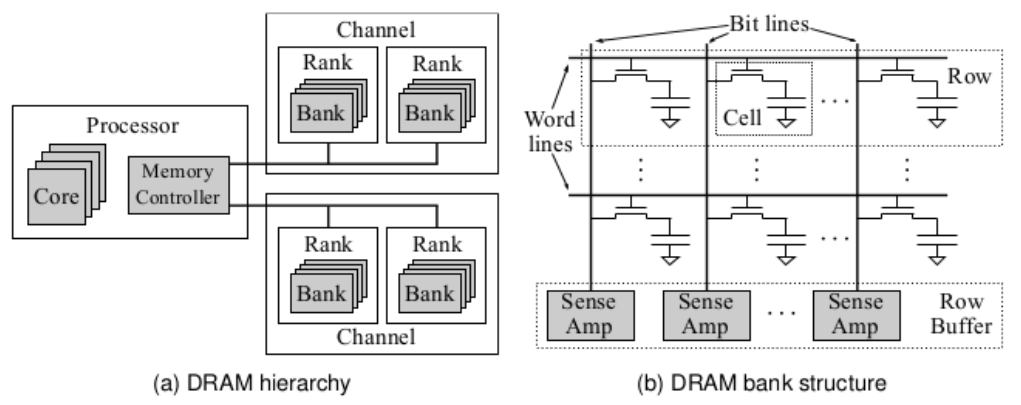
\includegraphics[width=8cm,height=3cm]{Dram_org.png}
\caption{Organisation of DRAM}
\label{fig3}
\end{figure}
\section{Overview of the Problem}\label{mot}
\noindent
Given a set of real time tasks, each with a deadline, the problem is to schedule the tasks on the DRAM such that the fewest 
number of tasks miss their deadlines.

$i^{th}$ task instance in a real time system, denoted by $\tau_{i}$ can be represented with the help of the following 
parameters -
\[\tau_{i} = (A_{i}, E_{i}, D_{i}, P_{i})\]
where $A_{i}$ denotes the arrival time of $i^{th}$ task instance, $E_{i}$ denotes worst case execution time of $i^{th}$ task instance,
$D_{i}$ denotes deadline of $i^{th}$ task instance, $P_{i}$ denotes the time interval after which the next task instance 
arrives.

We present our problem with the help of a motivating example.
\subsection{Motivating Example}
\noindent
Let us consider a simple DRAM with two banks, B0 and B1, each bank having a set of four rows. 
The bank mapping of the two banks are as follows -
\begin{itemize}
 \item Bank B0 contains four sets of rows. Row 0 (addr 0-addr 3), Row 1 (addr 4-addr 7), Row 2 (addr 8-addr 11) and 
 Row 3 (addr 12-addr 15).
 \item Bank B1 contains four sets of rows. Row 0 (addr 16-addr 19), Row 1 (addr 20-addr 23), Row 2 (addr 24-addr 27) 
 and Row 3 (addr 28-addr 31).
\end{itemize}
We consider that our DRAM follows open page policy, i.e., memory requests which result in row hit will be allowed to access 
the DRAM. We consider two tasks T1 and T2 arriving at the same time instant and scheduled according to EDF at the processor.
Each task consists of some CPU and Memory instructions. In this example, we have denoted the CPU instructions with $<$C$>$ and 
the Memory instructions as $<$M addr$>$, which denotes a memory instruction at address ``addr''. We consider the task 
specifications given in Table \ref{tab1}. Assume each CPU instruction takes 100 cycles to execute,
each memory instruction takes 300 cycles to execute when there is a row miss and 200 cycles to execute when there is a row hit.
Since tasks are scheduled according to EDF, T2 will be allowed to access the CPU earlier. A detailed picture of the 
waiting queue at the processor, the processor, the memory buffer, the memory and the status of T1 and T2 at different
cycles is described in Table \ref{tab2}. It can be inferred from this example, that due to address mapping policy, all the 
memory requests are mapped to Bank B1. Again, due to the open row policy, some of T1's memory requests although arrived 
earlier, could not get access to memory. As a result, T1 cannot complete its execution within its deadline. 

If T1's memory request is allowed to execute in Bank B0, then T1 can easily complete its execution within its deadline.
But executing a memory request in some other memory bank incurs a lot of overheads. We propose a novel method of bank aware 
partitioning based on a cost function calculated locally taking into account all the overheads so that the tasks can complete 
execution within deadline. We discuss our proposal in the following subsection.

\begin{table}[t]
\caption{Task Specifications}
\begin{center}
\scalebox{0.9}{
 \begin{tabular}{|c|c|c|c|}\hline
 \bf{Task}& \bf{Instructions}& \bf{Bank}& \bf{Deadline} \\ 
 \bf{ID}  &             & \bf{Mapping}&      \\ \hline
 T1 & C & & 1800 cycles \\
    & M 25 & Bank1-Row2 & \\
    & M 20 & Bank1-Row1 & \\
    & C & & \\
    & M 30 & Bank1-Row3 & \\
    & M 28 & Bank1-Row3 & \\ \hline
 T2 & C & & 1500 cycles \\
    & M 30 & Bank1-Row3 & \\
    & M 29 & Bank1-Row3 & \\
    & C & & \\
    & M 24 & Bank1-Row2 & \\ \hline
 \end{tabular}
 }
 \end{center}
\label{tab1}
\end{table}

\begin{table}[t]
\centering
\caption{A snapshot of the entire system at different cycles}
\scalebox{0.9}{
\begin{tabular}{|c|c|c|c|c|c|}\hline
\bf{Cycle}&\bf{Waiting}&\bf{Processor}&\bf{Memory}&\bf{Memory}&\bf{Status} \\ 
        &\bf{Queue}&              &\bf{Buffer}&             &\\ \hline
       0& T1       & T2           &           &          &\\ \hline
      99& T1       & T2           &           &          &\\ \hline
     100&          & T1           &           &T2 $<$M 30$>$& T2-Row\\ 
        &          &              &           &Bank1 Row 3& Miss\\ \hline
     199&          & T1           &           &T2 $<$M 30$>$&\\ 
        &          &              &           &Bank1 Row3&\\ \hline
     200&          &              & T1        &T2 $<$M 30$>$&\\
        &          &              &           &Bank1 Row3&\\ \hline
     399&         &              & T1        &T2 $<$M 30$>$&\\ 
        &          &              &           &Bank1 Row3&\\ \hline
     400&          &              & T1        &T2 $<$M 29$>$& T2-Row\\
        &          &              &           &Bank1 Row3& Hit\\ \hline
     599&          &              & T1        &T2 $<$M 29$>$& \\
        &          &              &           &Bank1 Row3&\\ \hline
     600&          & T2           &           &T1 $<$M 25$>$& T1-Row\\ 
        &          &              &           &Bank1 Row2& Miss\\ \hline
     899&          &              & T2        &T1 $<$M 25$>$& \\
        &          &              &           &Bank1 Row2&\\ \hline
     900&          &              & T1        &T2 $<$M 24$>$& T2-Row\\ 
        &          &              &           &Bank1 Row2& Hit\\ \hline
    1099&          &              & T1        &T2 $<$M 24$>$& T2-complete \\ 
        &          &              &           &Bank1 Row2& execution\\ \hline
    1100&          &              &           &T1 $<$M 20$>$& T1-Row \\ 
        &          &              &           &Bank1 Row1& Miss\\ \hline
    1399&          &              &           &T1 $<$M 20$>$&\\
        &          &              &           &Bank1 Row1&\\ \hline
    1400&          & T1           &           &          &\\ \hline
    1499&          & T1           &           &          &\\ \hline
    1500&          &              &           &T1 $<$M 30$>$& T1-Row\\ 
        &          &              &           &Bank1 Row3& Miss\\ \hline
    1799&          &              &           &T1 $<$M 30$>$& \\
        &          &              &           &Bank1 Row3&\\ \hline
    1800&          &              &           &T1 $<$M 28$>$& T1-Deadline \\ 
        &          &              &           &Bank1 Row3& Miss\\ \hline     
\end{tabular}
}

\label{tab2}
\end{table}

\subsection{Detailed Methodology}
\noindent
We have implemented a two level scheduler, one at the processor and the other at the memory controller. We have applied EDF to 
schedule tasks at the processor, i.e., tasks whose deadline is earliest is placed at the front of the priority queue and are 
allowed to execute first. But as the memory requests arrive at the DRAM controller, they are not executed in the order 
they are scheduled. Open page policy prioritizes those memory requests which result in row buffer hit of tasks. We propose 
to keep a set of extra memory banks which will not participate in address mapping. These extra memory banks are also known as
the reserved banks. We formulate a cost function based on some
known task parameters and schedule tasks based on that cost function. Cost function, $Cost_{ij}$, is the cost to execute 
$i^{th}$ instruction of $j^{th}$ task. We define another variable, $C_{ijk}$, which is the remaining time after execution
of $i^{th}$ instruction of $j^{th}$ task in $k^{th}$ bank (where it is actually mapped) and is given by-
\[C_{ijk} = D_{j} - (t_{ik} + e_{iw} + e_{ik} + e_{rem})\]\label{eq1}
where $D_{j}$ : the deadline of $j^{th}$ task,\\
$t_{ik}$ : the time to copy the $i^{th}$ instruction in $k^{th}$ bank,\\
$e_{iw}$ : the maximum waiting time of $i^{th}$ task in the memory buffer due to presence of other tasks infront of the 
$i^{th}$ instruction in the memory buffer,\\
$e_{ik}$ : the execution time of $i^{th}$ instruction in $k^{th}$ bank if there is a row miss/hit,\\
$e_{rem}$ : the worst case execution time required by the remaining instructions of $j^{th}$ task.

Similarly, $C_{ijk'}$ is defined as the remaining time after execution of $i^{th}$ instruction of $j^{th}$ task in one of the 
extra memory banks or the reserved banks, say k'. Our aim is to execute the $i^{th}$ instruction of $j^{th}$ task instance in the bank that allows us to 
have greater remaining time so that there is a lesser chance of having a deadline miss. This is determined with the help of the 
cost function $C_{ij}$ which is given by-

\[Cost_{ij} = C_{ijk} - C_{ijk'}\]

If $Cost_{ij}$ is greater than 0, we allow the task to execute in its own bank, otherwise we schedule it to execute in any one 
of the reserved set of banks. Algorithm \ref{alg1} explains our proposed method.

\begin{algorithm}[t]
   \caption {\textcolor{black}{Scheduling Policy at the Memory Controller}}
   \label{alg1}
    \begin{algorithmic}[1]
      \Function{SchedMemReq}{$Task$ $t$, Instruction $I$}\Comment{$t$ - Task, $I$ - $i^{th}$ memory instruction of task $t$}
       \State {$t_{ik}$ - time to copy $i^{th}$ instruction in $k^{th}$ bank}
       \State {$e_{iw}$ = maximum waiting time of $t$ due to tasks which are in the waiting queue ahead of $t$}
       \State {$e_{ik}$ = execution time of $i^{th}$ instruction in $k^{th}$ bank in case of a row hit/miss}
       \State {$e_{ik'}$ = execution time of $i^{th}$ instruction in its own bank in case of a row hit/miss}
       \State {$e_{rem}$ = worst case execution time of all the remaining instructions}
       \State {$C_{itk}$ = $t.deadline$ - ($t_{ik}$ + $e_{iw}$ + $e_{ik}$ + $e_{rem}$)}\Comment{$C_{itk}$ denotes the total time
       remaining after executing $i^{th}$ instruction of task $t$ in $k^{th}$ bank}
       \State {$C_{itk'}$ = $t.deadline$ - ($e_{iw}$ + $e_{ik'}$ + $e_{rem}$)}\Comment{$C_{itk}$ denotes the total time
       remaining after executing $i^{th}$ instruction of task $t$ in its own bank}
       \State {$Cost_{ij}$ = $C_{ijk}$ - $C_{ijk'}$}\Comment{$Cost_{ijk}$ denotes the cost incurred in the process}
       \If {$Cost_{ij}$ $>$ 0}
           \State {Schedule $t$ in its own bank}
       \Else
           \State {Schedule $t$ in some reserved banks}
       \EndIf
      \EndFunction  
    \end{algorithmic}
\end{algorithm}


\section{Implementation and Results} \label{imple}


\begin{table}[b]
\centering
\caption{List of Benchmark programs used as real time tasks}
\scalebox{0.9}{
\begin{tabular}{|c|c|c|c|} \hline
\bf{Benchmark} & \bf{Total}  & \bf{Memory} & \bf{Memory}\\ 
\bf{programs} & \bf{instructions} & \bf{Reads} & \bf{Writes} \\ \hline
bs & 179 & 32 & 32 \\ \hline
cnt & 295 & 52 & 43 \\ \hline
duff & 257 & 47 & 64 \\ \hline
fac & 164 & 24 & 24 \\ \hline
fibcall & 163 & 27 & 28 \\ \hline
insertsort & 189 & 36 & 30\\ \hline
lcdnum & 198 & 26 & 23 \\ \hline
ns & 245 & 31 & 40 \\ \hline
prime & 226 & 28 & 41 \\ \hline
res & 179 & 91 & 88 \\ \hline
\end{tabular}
}
\label{bench}
\end{table}




\begin{table}
\begin{flushleft}
\caption{Results on some of the Datasets}
\scalebox{0.9}{
 \begin{tabular}{|c|c|c|c|c|c|}\hline
 \bf{Dataset} & \bf{Number} & \bf{Number} & \bf{Rowsize} & \bf{Number} & \bf{Number} \\
 \bf{Number}  &  \bf{of}  & \bf{of}  & & \bf{of Task} & \bf{of Task} \\ 
         &  \bf{cycles} & \bf{Banks} &  & \bf{Miss}&\bf{Miss}  \\
         &        &       &    & \bf{(open-page}& \bf{(our} \\         
         &         &       &  & \bf{policy)}         &  \bf{method)}\\
 \hline Dataset I & 10,000 & 10 banks & 64B & 1 & 1 \\
 (fibcall.c,& 20,000 &          &     & 3 & 2 \\
  lcdnum.c,&30,000 &          &      & 4 & 3 \\
  fac.c)   &40,000 &          &      & 6 & 4 \\
           & 50,000 &        &       & 8 & 5 \\
           & 60,000 &        &      & 9 & 6 \\
           & 70,000 &        &      & 11 & 7 \\ \hline
           & 10,000 & 10 banks & 32B & 2 & 1 \\ 
           & 20,000 &        &       & 4 & 2 \\
           & 30,000 &        &       & 5 & 3 \\
           & 40,000 &        &       & 8 & 5 \\
           & 50,000 &        &       & 11 & 6 \\
           & 60,000 &        &       & 12 & 7 \\
           & 70,000 &        &       & 14 & 9 \\ \hline
 Dataset II & 10,000 & 19 banks & 64B & 3 & 0 \\
 (bs.c,     & 20,000 &         &      & 6 & 1 \\
  count.c   & 30,000 &         &      & 9 & 1 \\
  duff.c)   & 40,000 &         &      & 14 & 4 \\ \hline
            & 10,000 & 19 banks & 32B & 3 & 2 \\
            & 20,000 &          &     & 5 & 3 \\
            & 30,000 &          &     & 8 & 6 \\
            & 40,000 &          &     & 13 & 11 \\ \hline
 Dataset III & 10,000 & 15 banks & 64B & 2 & 1 \\
 (prime.c,   & 20,000 &          &     & 4 & 1 \\
  ns.c,      & 30,000 &          &     & 5 & 2 \\
  insertsort.c)& 40,000 &          &     & 8 & 3 \\ \hline
             &10,000 & 15 banks & 32B & 3 & 2 \\  
             & 20,000&          &     & 5 & 3 \\
             & 30,000&          &     & 6 & 4 \\
             & 40,000&          &     & 9 & 6 \\ \hline
 Dataset IV  & 10,000& 12 banks & 64B & 2 & 1 \\
 (lcdnum.c,  & 20,000 &         &     & 5 & 2 \\
  insertsort.c,& 30,000 &         &     & 7 & 4 \\
  fibcall.c) & 40,000 &         &     & 12 & 4 \\ \hline
             &10,000 & 12 banks & 32B & 3 & 2 \\
             & 20,000 &         &     & 6 & 4 \\
             & 30,000 &         &     & 9 & 6 \\
             & 40,000 &         &     & 14 & 11\\ \hline  
 \end{tabular}
 }
\end{flushleft}
\label{Data_results}
\end{table}


\noindent
Our end to end implementation consists of two main parts. The first part consists of trace generation from benchmark programs 
of the Malardalen WCET benchmark~\cite{gustafsson2010malardalen}. We executed our benchmark programs on an X-86 architectural 
platform to generate X-86 instructions. Table~\ref{bench} gives a description of the benchmark programs in detail. 
In our implementation, the arrival time (A) of each task is randomly generated. The execution time of a task(E) is actually the 
sum of execution time of all the instructions in the worst case. The period of each task (P) is randomly generated with the 
condition that it should 
be greater than the worst case execution time. We have considered the deadline of a task instance (D) to be equal to 
the period after which the next task instance arrives. Thus at a particular time instant only one task 
instance of a task actually executes in the system. 
%A diagrammatic view of our trace generation is shown in Fig \ref{fig5}. 
The final part deals with the end to end simulation. 
We have considered a uni-processor system, where tasks are scheduled according to EDF at the processor. Whenever a memory 
request arrives, a context switch occurs at the CPU and the memory request waits in the memory buffer. The memory controller 
then selects a request from the memory buffer based on our proposed algorithm and executes a task in memory. Our results were
generated by varying the number of banks and the size of row in each bank. In all the cases, we have assumed that we have a set 
of two extra banks which do not participate in address mapping. We have 
implemented our own end-to-end simulator and have compared our results with existing state-of-the-art DRAM controllers. 
Table \ref{Data_results} shows a comparative analysis of existing DRAM controllers following open-page policy vs our proposed DRAM 
controller. We have generated some dataset from the benchmark programs of the Malardalen WCET benchmark. We have run each dataset
upto certain number of cycles by varying the number of memory banks. We have also varied the size of each row in a memory bank.
In Table \ref{Data_results}, column I shows the programs in each dataset, column II shows the number of cycles upto which we ran our 
experiments, column III shows the number of banks in the memory module we worked on, column IV shows the size of row in each 
bank, column V shows the number of misses in DRAM with open-page policy and column VI shows the number of misses we achieved by using 
our scheduling algorithm at the DRAM controller.



%\begin{figure}
% \centering
%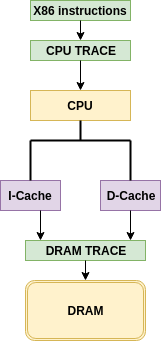
\includegraphics[width=3.5cm,height=4.2cm]{TRACE.png}
% \caption{Overview of Trace Generation}
% \label{fig5}
%\end{figure}






\section{Conclusion} \label{con}
\noindent
In this paper, we present the problem of open page policy in state-of-the-art DRAM controllers and the problem in 
using these DRAMs in real time systems. In real time systems, though the real time tasks are scheduled based on some priority
based scheduling algorithms at the processor, the tasks are not executed in the same order in the memory due to prioritization
of some other tasks at the DRAM controller. This becomes a bottleneck to guarantee 
completion of all real time tasks within their deadline. Finally, we proposed a scheduling algorithm at the DRAM which 
schedules the tasks based on a cost function evaluated on the basis of some local task parameters. We implemented an 
end-to-end simulator for the same and generated our results on the Malardalen WCET benchmark programs.


\section{Acknowledgement}
This work was partially funded by a research grant from De-
fence Research and Development Organization, Government 
of India awarded to Indian Statistical Institute.

\scriptsize
\bibliographystyle{plain}
\bibliography{bare_conf}
\end{document}


